\documentclass[english]{article}
\usepackage[utf8]{inputenc}
\usepackage[T1]{fontenc}
\usepackage{afterpage}
\usepackage{graphicx}
\usepackage{geometry}
\usepackage{amsmath}
\usepackage{babel}
\usepackage{float}
\usepackage{multirow}
\usepackage{array}
\newcolumntype{C}{>{\centering\arraybackslash}m{2cm}}
% Add in specific class to use \subsubsubsection, \paragraph, \subparagraph
\usepackage{titlesec}
\titleclass{\subsubsubsection}{straight}[\subsection]
\newcounter{subsubsubsection}[subsubsection]
\renewcommand\thesubsubsubsection{\thesubsubsection.\arabic{subsubsubsection}}
\renewcommand\theparagraph{\thesubsubsubsection.\arabic{paragraph}} % optional; useful if paragraphs are to be numbered
\titleformat{\subsubsubsection}
  {\normalfont\normalsize\bfseries}{\thesubsubsubsection}{1em}{}
\titlespacing*{\subsubsubsection}
{0pt}{3.25ex plus 1ex minus .2ex}{1.5ex plus .2ex}
\makeatletter
\renewcommand\paragraph{\@startsection{paragraph}{5}{\z@}%
  {3.25ex \@plus1ex \@minus.2ex}%
  {-1em}%
  {\normalfont\normalsize\bfseries}}
\renewcommand\subparagraph{\@startsection{subparagraph}{6}{\parindent}%
  {3.25ex \@plus1ex \@minus .2ex}%
  {-1em}%
  {\normalfont\normalsize\bfseries}}
\def\toclevel@subsubsubsection{4}
\def\toclevel@paragraph{5}
\def\toclevel@paragraph{6}
\def\l@subsubsubsection{\@dottedtocline{4}{7em}{4em}}
\def\l@paragraph{\@dottedtocline{5}{10em}{5em}}
\def\l@subparagraph{\@dottedtocline{6}{14em}{6em}}
\makeatother
\setcounter{secnumdepth}{4}
\setcounter{tocdepth}{3}
\geometry{left=1.5in, right=1.5in, top=1in, bottom=1.25in}
\titleformat{\section}{\clearpage\normalfont\Large\bfseries}{\thesection}{1em}{}
\usepackage{hyperref}
\hypersetup{
    colorlinks=true,
    linkcolor=black,
    filecolor=magenta,      
    urlcolor=blue,
    pdfpagemode=FullScreen,
}

\begin{document}

\begin{titlepage}
\centering

\vspace{4cm} 

\Huge

Üzleti Intelligencia

\vspace{2cm} 

\Large

Megerősítéses tanulás - beadandó feladatok

\vspace{0.5cm}

2023 % Dátum

\vspace{2cm} 

\normalsize

A feladatok 1-3 skálán vannak osztályozva nehézség szerint, ahol 1 a legkönnyebb és 3 a legnehezebb. A feladatok véletlenszerűen sorsolódnak ki a 6. gyakorlaton. A feladatok beadása Coospace felületen történik, ahol csak egy linket kell beküldeni, ami a feladatot megvalósító Git tárhelyre mutat. Késő beadás nem lehetséges, a dátum beadásakor feltöltött anyagok fognak leosztályozásra kerülni. Minden további információ a tantárgyi útmutatóban és az órán elhangzottakban találhatóak.
\end{titlepage}

\section{Duna}
Az ügynök Esztergomban áll, és olyan gyorsan kell eljutnia Pestre, amennyire csak lehet. Két út van, amelyekkel elhagyhatja a várost, az 10-es és 11-es út Mindkét út különböző helyre vezet.

Miután megérkezett Budára, két hídon juthat át a Duna folyón, hogy eljusson Pestre. A forgalom kiszámíthatatlan, így előfordulhat, hogy a hídon amit választott forgalmi dugó alakul ki.

Néha pedig átirányítódik a másik hídra annak ellenére, hogy a másik útvonalat vagy hidat választotta.

A cél az, hogy olyan stratégiát találjon az ügynök, ami a leghamarabb eljuttatja a céljához. A jutalmak a negatív időt jelentik, amelyre szüksége van az adott út/híd átlépéséhez.

Az $A$, $B$, $C$  állapotokhoz és minden cselekvéshez a jutalom a következőképpen számolódik ki:
\[R(s,a) = 
\begin{cases}
_{\textit{Ha dugó van}}^{\textit{Ha nincs dugó}} & _{R(s,\textit{dugó})}^{R(s,\textit{norm})}
\end{cases}
\]

Előfordulhat, hogy az ügynök választ egy irányt, de átirányítják a másikra. Tehát ha $P(s,a,s') = 0.9$, tehát $90\%$ valószínűséggel abba az irányba megy, amit választott, de $10\%$ valószínűséggel átirányítják a másik útra.

\begin{center}
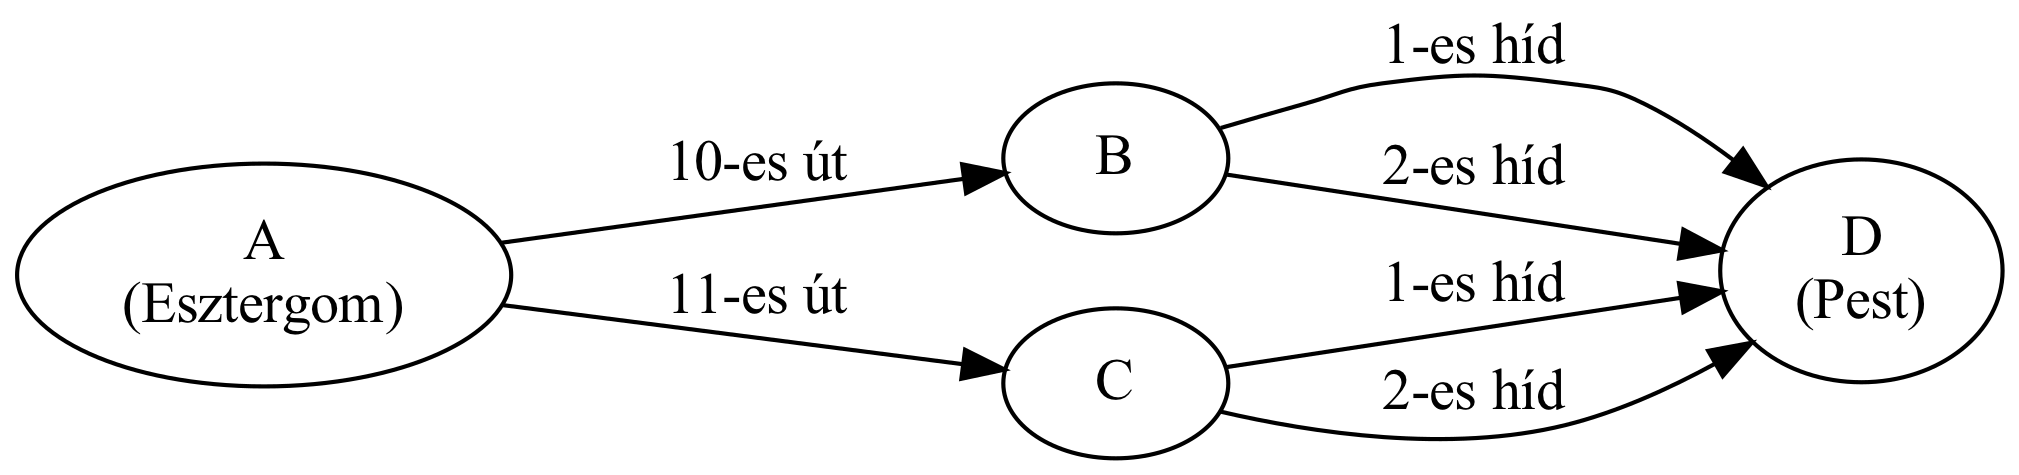
\includegraphics[width=\textwidth, keepaspectratio]{graphs/1_duna.png}
\end{center}

\subsubsection*{A környezet dinamikája ($P(s,a,s'), R(s,a,s')$):} 
$P(A,10,B)=0.79$, $P_\text{dugó}(A,10,B)=0.9$, $R_\text{dugó}(A,10,B)=-60$, $R_\text{norm}(A,10,B)=-21$\\
$P(A,11,C)=0.89$, $P_\text{dugó}(A,11,C)=0.56$, $R_\text{dugó}(A,11,C)=-44$, $R_\text{norm}(A,11,C)=-1$\\
$P(B,1,D)=0.84$, $P_\text{dugó}(B,1,D)=0.43$, $R_\text{dugó}(B,1,D)=-20$, $R_\text{norm}(B,1,D)=-4$\\
$P(B,2,D)=0.7$, $P_\text{dugó}(B,2,D)=0.84$, $R_\text{dugó}(B,2,D)=-40$, $R_\text{norm}(B,2,D)=-11$\\
$P(C,1,D)=0.98$, $P_\text{dugó}(C,1,D)=0.75$, $R_\text{dugó}(C,1,D)=-65$, $R_\text{norm}(C,1,D)=-5$\\
$P(C,2,D)=0.77$, $P_\text{dugó}(C,2,D)=0.53$, $R_\text{dugó}(C,2,D)=-58$, $R_\text{norm}(C,2,D)=-10$\\

\subsection{Dinamikus programozás}
Oldja meg a problémát dinamikus programozással. Ehhez tartozóan implementálja a politika iteráció eljárását (politika kiértékelés, politika javítás). Futtassa a szimulációt adott konvergencia kritériumig. Mutassa meg, hogy az ügynök megtanulta optimalizálni a jutalmat. Írja le röviden az eljárás elméleti alapjait és a saját tapasztalatait egy Jupyter markdown cellában

\subsection{Sztochasztikus becslés}
Oldja meg a problémát sztochasztikus becsléssel. Ehhez tartozóan implementálja a Monte Carlo és időbeli különbségek politika keresési eljárásait. Futtassa a szimulációt adott konvergencia kritériumig. Mutassa meg, hogy az ügynök megtanulta optimalizálni a jutalmat. Írja le röviden az eljárás elméleti alapjait és a saját tapasztalatait egy Jupyter markdown cellában


\end{document}
















